\chapter{Introduction}

%- Intro biology
%- beskrivelse af opgaven
%- beskrivelse af batbox
%- (beskriv streaming idea)
% Link: http://www.bats.org.uk/pages/publications_and_resources.html

% as everything is considered as stream, it becomes naturally to also do online processing on th esound stream, and take the output as video streams(waterfall spectrogram)
% \todo{Set the scene - publishers/subscribers, define host, nodes etc.}
\section{Users}

\begin{itemize}
	\item Biologists
	\item Developers(users, Thor)
	\item Developers(Code, John)
	\item Supervisors
	\item Backend developers
\end{itemize}

\section{Use Cases}
\newpage
\subsection{Porpoise}
The biology department in Keerteminde conducts experiments with porpoises in order to gain an understanding of how their subsonic echolocation works. The general testsetup is depicted in figure \ref{usecase:porpoise_experiment1}.
\begin{figure}[!h]
    \centering
	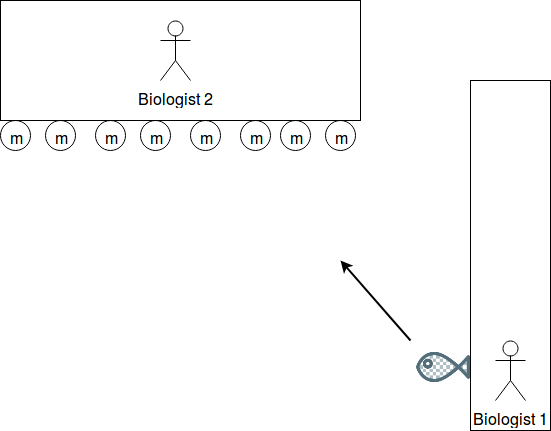
\includegraphics[width=\textwidth]{figures/porpoise_experiment1}
	\caption{Depict testsetup of porpoise echolocalization. The two boxes indicate pierses, each with a biologist. On the piers with biologist 2, 8 hydrophones are mounted.}\label{usecase:porpoise_experiment1}
\end{figure}


Figure \ref{usecase:porpoise_experiment1} shows a porpoise swimming in a basin close to \textit{Biologist 1}. \todo{Make sketch smaller, add bait near biologist 2, add piers label, batbox}
%The microphone recording system is mounted on a piers on which \textit{biologist 2} is located.
When \textit{Biologist 2} throws bait in the basin, the porpoise will swim torwards the bait while emitting high frequency, narrow band clicks, in order to swim in the direction of the bait.
Since 8 microphones are mounted near the bait on piers2, the recordingsystem is able to record the clicks emitted by the porpoise. This experiment exists in different variations where, for instance, different materials are mounted between the bait and the porpoise that tampers with the porpoise's clicks and hearing. The experiments are conducted using one batbox with 8 hydrophones.

\todo{Add extra sensors to system: Temperature, salinity and pH from the ocean}

These experiments use \textit{Trigger recordings} and \textit{Long recordings} as described in section \ref{sec:usecase:triggerrecording} and \ref{sec:usecase:longrecording} respectively.

\subsection{Bats}
The biologists at SDU do experiments with bats to gain knowledge about how bats use their echolocation, where bats live, and where they live in the nature.
Some of the experiments are conducted as described in section \ref{sec:usecase:porpoise} with porpoises. Instead of doing the experiments in water, they are conducted in a batcage showed in figure \ref{fig:usecase:batcage}. When the bats fly towards the bait, the biologist can create a recording using the trigger mechanism, as described in \ref{sec:usecase:triggerrecording}.

\begin{figure}[!h]
    \centering
    \begin{subfigure}[b]{0.45\textwidth}
        \includegraphics[width=\textwidth]{figures/batcage_cross}
        \caption{Figure of batcage with existing system's microphone mount}
        \label{fig:gull}
    \end{subfigure}
    ~ %add desired spacing between images, e. g. ~, \quad, \qquad, \hfill etc. 
    %(or a blank line to force the subfigure onto a new line)
    \begin{subfigure}[b]{0.45\textwidth}
        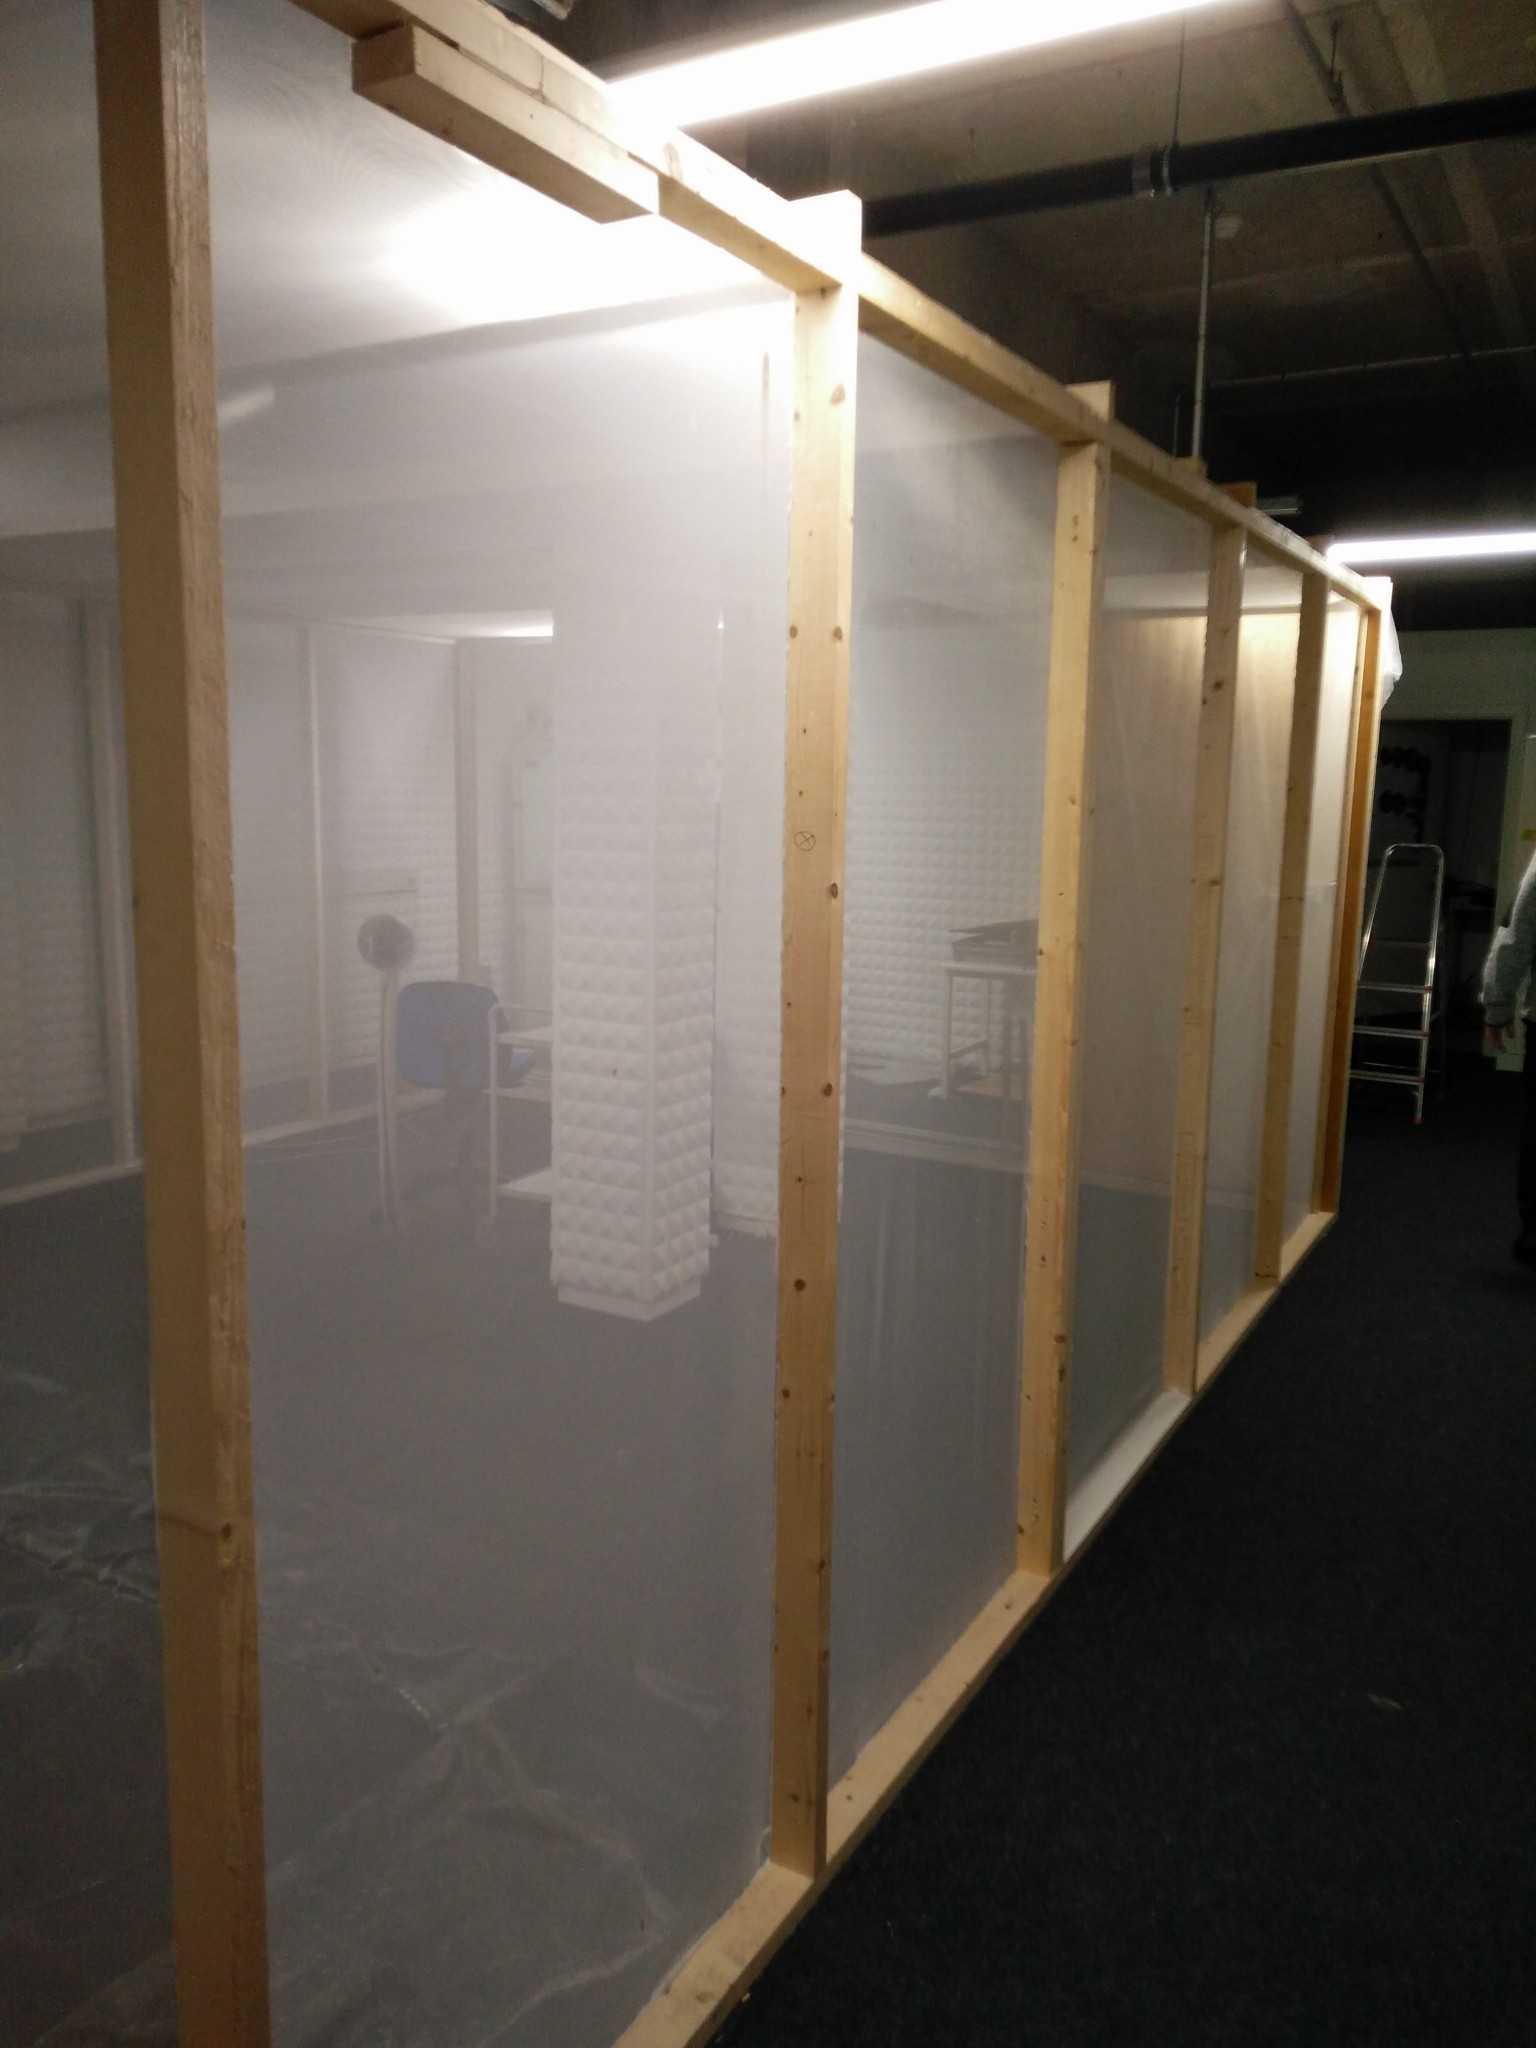
\includegraphics[width=\textwidth]{figures/batcage}
        \caption{Figure of the opposite end of the batcage}
        \label{fig:mouse}
    \end{subfigure}
    \caption{Pictures of batcage}\label{fig:usecase:batcage}
\end{figure}

Another set of experiments are conducted in panama. 8 microphones are mounted in a tree, in order to investigate which bat species live in the forest. As the microphones and the batbox is mounted in a forest, the batbox is running on battery. Due to the location of the recording system in a forest, it's cumbersome to get physical access to the system, to do maintenance like replacing battery, harddrives etc. The system do periodically \textit{short recordings} as described in section \ref{sec:usecase:shortrecordings}. 

A third experiment is done in Odense where the new hospital will be build.
%The idea is to investigate how the new hospital will affect the bats living in the area.
The idea is to put op N batboxes, each with 8 microphones in the area where the hospital will be build to get more knowledge about the bats that live in the area. During the conduct of the hospital and after the hospital has been build, the biologists want to know if the behaviour of bats have changed. The system should only do recordings in the nightly hour as bats are not active during daytime. This is described in section \ref{sec:usecase:shortrecordings}.

The biologists also have interest in mounting a batbox with a microphone on drones. An experiment is to manually steer a drone near a group of flying bats, to gain knowledge about how bats behave in the air, which species fly at different heights etc. This should in the future be automated such that two drones, each with 8 microphones and a batbox can point in the direction of the group of bats. In order to maintain the heading, the drones should emulate being a drone by emitting ultrasonic sounds which is then recorded by the microphones. The trigger recordings must be minimum 30 ms. To do this, processing of the recordings must be done online, as described in section \ref{sec:usecase:online}.
\todo{Question: App. where drones use echolocation?}
These experiments require long recordings as described in section \ref{sec:usecase:longrecording} in order to record while the drone is in the air and triggered-recording as described in section \ref{sec:usecase:triggerrecordings} to listen for subsonic replies emitted by the drone.

\subsection{Frogs}
biologists also have interest in recording frogs, in order to learn more about their vocalization. Frogs use advanced techniques to synchronize with other frogs, so they alternate vocalization to increase their change of being heard be females frogs. Further more they use techniques where they do vocalizing near a bigger male frog to amplify their vocalization to, as before, increase their change of getting hear by female frogs. Figure \ref{fig:usecase:frogs} shows an illustration of frogs vocalizing around a lake. Experiments are usually conducted by mounting 8 microphones and 1 batbox close to a lake. The system is running on battery and requires recording to be done in predefined period of time during daytime. This system requires short recordings as described in section \ref{sec:usecase:shortrecordings}

\missingfigure{Frogs + lake}



\subsection{Zebra Finches}
Biologists use Zebra Finches for investigating vocalization, as the Zebra finch has a stereotypical sound. Especially the tutoring session between a young bird and its father has been investigated thoroughly. In an experiment, a teleconference system for birds has been build. The two birds are physically isolated in boxes,
but can communicate via cameras, screens, microphones and speakers. One batbox has been used, where 1 microphone is placed in each of the two boxes.\citep{larsen2016system}
Figure \ref{fig:usecases:zebra:overview} shows the conceptual design of the experiment:

\begin{figure}[h!]
	\centering
	
\includegraphics[width=0.6\textwidth]{figures/zebrafinches_experiment1.png}
	\caption{Pictures of experiment with zebra finches where only microphones, batbox and speakers are depicted}\label{fig:usecases:zebra:overview}
\end{figure}
It should be noted, that only two microphones are in use in this system.
As the system is designed to replay tutoring sessions from previous experiments, it is required that the system can replay recordings.
The system uses long recordings as described in section \ref{fig:usecase:longrecording}.


\begin{figure}
    \centering
    \begin{subfigure}[b]{0.3\textwidth}
        
\includegraphics[width=\textwidth]{figures/recording_trigger.png}
        \caption{Trigger recording illustrated}
        \label{fig:usecase:triggerrecording}
    \end{subfigure}
    ~ %add desired spacing between images, e. g. ~, \quad, \qquad, \hfill etc. 
      %(or a blank line to force the subfigure onto a new line)
    \begin{subfigure}[b]{0.3\textwidth}
        
\includegraphics[width=\textwidth]{figures/recording_long.png}
        \caption{Long recording illustrated}
        \label{fig:usecase:longrecording}
    \end{subfigure}
    ~ %add desired spacing between images, e. g. ~, \quad, \qquad, \hfill etc. 
    %(or a blank line to force the subfigure onto a new line)
    \begin{subfigure}[b]{0.3\textwidth}
        
\includegraphics[width=\textwidth]{figures/recording_short.png}
        \caption{Short recording illustrated}
        \label{fig:usecase:shortrecording}
    \end{subfigure}
    \caption{Illustration of the three types of recordings}\label{fig:usecase:recordingtypes}
\end{figure}
\subsection{Long Recordings}
Long recordings are used in experiments where it is required to do continuous recordings for theoretically indefinitely. Long recordings are used where either storage is always available or the local attached storage can be replaced when out of space. A long recording is depicted in figure \ref{fig:usecase:longrecording}.

\subsection{Trigger Recordings} 
Trigger recordings are used in experiments where it potentially takes a long time before the event of interest is happening. By using a trigger recording, the recording can be triggered after the event has happened, but where the event is saved in the recording. In figure \ref{fig:usecase:triggerrecording} two microphones are depicted with respect to time. When the system receives a trig, it will export the recording to the the biologist, starting at $trig-pre$ to $trig+post$. The duration of the recording will therefore be $pre+post$. The trig is usually received by a press on a button.

\subsection{Short Recordings}
Short recordings are used when the storage is limited or the batbox is not always powered up due to power constrains such as the batbox is running on battery. The start of the recording and duration must be specified such that the biologists can key in when the recordings should be conducted.
A short recording is depicted in figure \ref{fig:usecase:shortrecording}.

\subsection{Data Analysis}
Analysis of recordings are usually done online, offline or as batch processing.
\subsubsection{Online}\label{sec:usecase:online}
Online processing is when the processing is happening while the experiment is conducted. This means the recordings are not saved for later processing, but used as recordings are generated.

\subsubsection{Offline}
Offline analysis is used in most use-cases where the recordings are saved to local storage. The processing of the recordings can be done when the local storage drive is brought back from the test-location.

\subsubsection{Batch Processing}
Batch processing is also happening offline, but in this case the recordings are exported as sound files, which can be used on a supercomputer such as Abacus. The different between offline and Batch Processing is the fact, that in offline-analysis, the format of the recordings is raw and requires pre-processing.

\subsection{Overall Idea}
\subsection{Insert figures}


\section{Existing System}

\begin{figure}[h!]
	\centering
	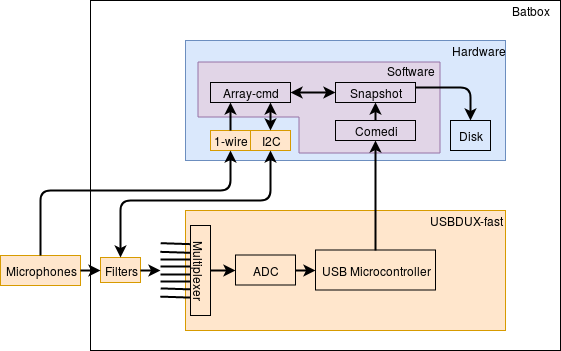
\includegraphics[width=1\textwidth]{figures/existing-system-overview.png} 
	\caption{Overview of existing system}\label{fig:existingsystem:overview}
\end{figure}




\subsection{Current setup}

As shown in section <Use-cases>, the existing system comprises of the following nodes:

snapchot is responsible for getting the auto from the usbdux/comedi module and writing the samples into files. When snapshot is initialized, it will record samples, however data is only saved to a circular buffer until it is told to write the buffer into a file. The snapshot will save part of the circular buffer to a file when it receives a “snap” command. This gives the ability to get a recording, consisting of data from a predefined time before it receives the “snap” command. Snapshot is designed to not miss out samples from the ADC.

grab has overlapping responsibility with snapshot, however: grab outputs samples to stdout and not by writing to any files. Furthermore, the implementation of the grab node is much more simple, as it has no need to maintain a circular buffering and thereby implement less memory management. If the consuming process blocks its stdin, grab will loose samples.

snapchat is responsible for communicating with snapchot and/or array-cmd depending on the application. Snapshot is run from CLI where it takes its input as parameters, and outputs by connecting to the snapshot/array-cmd.

cmd-arrays responsibilities are listed below:
Setting up the usbdux 
Handles GPIO to HMI
Saving meta-data for recordings
Determine mode of operation
Handling uuid generation
Handling recording paths
Handling connected microphones.
Being the interface to the system.
UDP + ZMQ
Hardware communication with:
LTC2637(DAC) over I2C
See flowchart of array-cmd.

trig instructs the snapshot when to do a snapshot by constructing and sending a “snap” command to either cmd-array or snapchat.

array is a script that hides the complexity of the system to ease the interface for the biologists. It is capable of initializing the system, listing connected microphones, setting options on the microphones, starting/stopping recordings etc.

Hardware - trigger line(master/slave setups)
Communication between nodes.
The interface to the recording system is either UDP or ZMQ using request/reply-pattern. Communication between the demons and CLI tools is ZMQ. Communication between threads in snapshot is also using ZMQ, however using push-patterns as ZMQ is used to do logging from busy threads.

Startup and supervision
All demons are run under supervision from the debian runit package. The runit package is both responsible for starting the nodes during startup, but also to keep the nodes running in case one of them crashes. Since runit does not provide any control of the order of startup, some fiddling has been made in order to start the snapshot and array-cmd in the proper order. From array-cmd’s run file, it tells snapshot’s supervisor, to start running.

Table of running/non-running processes.


Node name
Impl.Language
Running one-shot
Running forever
Running when used(long term)
snapshot




X


snapchat


X




grab






X
trig


X
X
X
array-cmd




X




Requirements:
Add other types of sensors (GPS, humidity, temp etc.)
Send recordings to backend when PI is online
The PI should not require internet to do recordings
Support for different hardware versions of the batbox.
Software should run on RPI
Snapshot should also be able to run on Intel in cases where powerfull enough RPI is not available.




Move files to more sensible structure
Describe different hardware versions as this makes up requirement for probing hardware

\todo{Describe and make diagrams of how to userlands tools talk through comedi modules to hardware}
\subsection{Hardware versions}
Version 1
Version 2A
Version 2B
Drone
\todo{Describe hardware. Make diagrams of the connected components}

\section{Streaming}

\subsection{Uses cases with Streaming}
\todo{Insert figures from first-handed document describing how the streaming idea applies to the different use cases}
%\myparagraph{Interface}
%As biologists are the typical user of the system, a userfriendly webinterface should be provided. Designing and implementing this is out of the scope of the report. However, it is kept in mind

